% Options for packages loaded elsewhere
% Options for packages loaded elsewhere
\PassOptionsToPackage{unicode}{hyperref}
\PassOptionsToPackage{hyphens}{url}
\PassOptionsToPackage{dvipsnames,svgnames,x11names}{xcolor}
%
\documentclass[
  10pt,
]{article}
\usepackage{xcolor}
\usepackage[margin=2cm]{geometry}
\usepackage{amsmath,amssymb}
\setcounter{secnumdepth}{5}
\usepackage{iftex}
\ifPDFTeX
  \usepackage[T1]{fontenc}
  \usepackage[utf8]{inputenc}
  \usepackage{textcomp} % provide euro and other symbols
\else % if luatex or xetex
  \usepackage{unicode-math} % this also loads fontspec
  \defaultfontfeatures{Scale=MatchLowercase}
  \defaultfontfeatures[\rmfamily]{Ligatures=TeX,Scale=1}
\fi
\usepackage{lmodern}
\ifPDFTeX\else
  % xetex/luatex font selection
\fi
% Use upquote if available, for straight quotes in verbatim environments
\IfFileExists{upquote.sty}{\usepackage{upquote}}{}
\IfFileExists{microtype.sty}{% use microtype if available
  \usepackage[]{microtype}
  \UseMicrotypeSet[protrusion]{basicmath} % disable protrusion for tt fonts
}{}
\makeatletter
\@ifundefined{KOMAClassName}{% if non-KOMA class
  \IfFileExists{parskip.sty}{%
    \usepackage{parskip}
  }{% else
    \setlength{\parindent}{0pt}
    \setlength{\parskip}{6pt plus 2pt minus 1pt}}
}{% if KOMA class
  \KOMAoptions{parskip=half}}
\makeatother
% Make \paragraph and \subparagraph free-standing
\makeatletter
\ifx\paragraph\undefined\else
  \let\oldparagraph\paragraph
  \renewcommand{\paragraph}{
    \@ifstar
      \xxxParagraphStar
      \xxxParagraphNoStar
  }
  \newcommand{\xxxParagraphStar}[1]{\oldparagraph*{#1}\mbox{}}
  \newcommand{\xxxParagraphNoStar}[1]{\oldparagraph{#1}\mbox{}}
\fi
\ifx\subparagraph\undefined\else
  \let\oldsubparagraph\subparagraph
  \renewcommand{\subparagraph}{
    \@ifstar
      \xxxSubParagraphStar
      \xxxSubParagraphNoStar
  }
  \newcommand{\xxxSubParagraphStar}[1]{\oldsubparagraph*{#1}\mbox{}}
  \newcommand{\xxxSubParagraphNoStar}[1]{\oldsubparagraph{#1}\mbox{}}
\fi
\makeatother


\usepackage{longtable,booktabs,array}
\newcounter{none} % for unnumbered tables
\usepackage{calc} % for calculating minipage widths
% Correct order of tables after \paragraph or \subparagraph
\usepackage{etoolbox}
\makeatletter
\patchcmd\longtable{\par}{\if@noskipsec\mbox{}\fi\par}{}{}
\makeatother
% Allow footnotes in longtable head/foot
\IfFileExists{footnotehyper.sty}{\usepackage{footnotehyper}}{\usepackage{footnote}}
\makesavenoteenv{longtable}
\usepackage{graphicx}
\makeatletter
\newsavebox\pandoc@box
\newcommand*\pandocbounded[1]{% scales image to fit in text height/width
  \sbox\pandoc@box{#1}%
  \Gscale@div\@tempa{\textheight}{\dimexpr\ht\pandoc@box+\dp\pandoc@box\relax}%
  \Gscale@div\@tempb{\linewidth}{\wd\pandoc@box}%
  \ifdim\@tempb\p@<\@tempa\p@\let\@tempa\@tempb\fi% select the smaller of both
  \ifdim\@tempa\p@<\p@\scalebox{\@tempa}{\usebox\pandoc@box}%
  \else\usebox{\pandoc@box}%
  \fi%
}
% Set default figure placement to htbp
\def\fps@figure{htbp}
\makeatother





\setlength{\emergencystretch}{3em} % prevent overfull lines

\providecommand{\tightlist}{%
  \setlength{\itemsep}{0pt}\setlength{\parskip}{0pt}}



 


\usepackage{graphicx}
\usepackage{amsmath}
\usepackage{booktabs}
\usepackage{float}
\usepackage{caption}
\usepackage{setspace}
\usepackage{fancyhdr}
\captionsetup{font=small}
\singlespacing
\pagestyle{fancy}
\fancyhf{}
\fancyfoot[C]{\thepage}
\makeatletter
\@ifpackageloaded{caption}{}{\usepackage{caption}}
\AtBeginDocument{%
\ifdefined\contentsname
  \renewcommand*\contentsname{Table of contents}
\else
  \newcommand\contentsname{Table of contents}
\fi
\ifdefined\listfigurename
  \renewcommand*\listfigurename{List of Figures}
\else
  \newcommand\listfigurename{List of Figures}
\fi
\ifdefined\listtablename
  \renewcommand*\listtablename{List of Tables}
\else
  \newcommand\listtablename{List of Tables}
\fi
\ifdefined\figurename
  \renewcommand*\figurename{Figure}
\else
  \newcommand\figurename{Figure}
\fi
\ifdefined\tablename
  \renewcommand*\tablename{Table}
\else
  \newcommand\tablename{Table}
\fi
}
\@ifpackageloaded{float}{}{\usepackage{float}}
\floatstyle{ruled}
\@ifundefined{c@chapter}{\newfloat{codelisting}{h}{lop}}{\newfloat{codelisting}{h}{lop}[chapter]}
\floatname{codelisting}{Listing}
\newcommand*\listoflistings{\listof{codelisting}{List of Listings}}
\makeatother
\makeatletter
\makeatother
\makeatletter
\@ifpackageloaded{caption}{}{\usepackage{caption}}
\@ifpackageloaded{subcaption}{}{\usepackage{subcaption}}
\makeatother
\usepackage{bookmark}
\IfFileExists{xurl.sty}{\usepackage{xurl}}{} % add URL line breaks if available
\urlstyle{same}
\hypersetup{
  pdftitle={Práctica arboles de desición},
  pdfauthor={Ismael Maximiliano De Los Santos Huesca},
  colorlinks=true,
  linkcolor={blue},
  filecolor={Maroon},
  citecolor={Blue},
  urlcolor={Blue},
  pdfcreator={LaTeX via pandoc}}


\title{Práctica arboles de desición}
\author{Ismael Maximiliano De Los Santos Huesca}
\date{2026-10-21}
\begin{document}
\maketitle

\begin{titlepage}

    % Logos alineados izquierda y derecha
    \begin{minipage}{0.45\textwidth}
        \raggedright
        
\includegraphics[width=7cm]{Logo_UNAM.png}
    \end{minipage}
    \hfill
    \begin{minipage}{0.45\textwidth}
        \raggedleft
        
\includegraphics[width=3.4cm]{Logo_LCG.png}
    \end{minipage}

    \centering
    \vspace*{2cm}

    {\Huge\bfseries Práctica comparación DT, RF y SVM \par}
    \vspace{2cm}
    
    {\Large Data Science \par}
    \vspace{1cm}
    
    {\Large De Los Santos Huesca Ismael Maximiliano \par}
    \vspace{1cm}

    {\Large Dr. Carlos Mendez\par}
    \vspace{1cm}
    
    {\Large Fecha: 21 Octubre 2026 \par}
    
    \vfill

\end{titlepage}


\section{Planteamiento}\label{planteamiento}

Esta práctica pretende evaluar el desempeño de 3 algoritmos de machine
learning (ML) (Decision Tree, Random Forest y SVM) a partir de un
dataset con una variable objetivo de interés y 12 características que se
pueden utilizar para el entrenamiento del modelo. De estas, se
utilizaron 11 variables predictoras debido a la redundancia de la edad
de los 70000 individuos en el dataset, por lo que se optó por conservar
la edad en años y eliminar la columna de días.

\begin{table}[!h]
\centering
\caption{\label{tab:tabla_data_set}Data set con todas las variables presente en el mismo}
\centering
\resizebox{\ifdim\width>\linewidth\linewidth\else\width\fi}{!}{
\begin{tabular}[t]{lrrrrrrrrrrrr}
\toprule
  & age\_year & gender & height & weight & ap\_hi & ap\_lo & cholesterol & gluc & smoke & alco & active & cardio\\
\midrule
0 & 50.39178 & 2 & 168 & 62 & 110 & 80 & 1 & 1 & 0 & 0 & 1 & 0\\
1 & 55.41918 & 1 & 156 & 85 & 140 & 90 & 3 & 1 & 0 & 0 & 1 & 1\\
2 & 51.66301 & 1 & 165 & 64 & 130 & 70 & 3 & 1 & 0 & 0 & 0 & 1\\
3 & 48.28219 & 2 & 169 & 82 & 150 & 100 & 1 & 1 & 0 & 0 & 1 & 1\\
4 & 47.87397 & 1 & 156 & 56 & 100 & 60 & 1 & 1 & 0 & 0 & 0 & 0\\
\addlinespace
8 & 60.03836 & 1 & 151 & 67 & 120 & 80 & 2 & 2 & 0 & 0 & 0 & 0\\
\bottomrule
\end{tabular}}
\end{table}

\section{Preparación de datos y
División}\label{preparaciuxf3n-de-datos-y-divisiuxf3n}

El dataset fue dividido en conjuntos de entrenamiento (para ser aplicado
mediante validación cruzada) y prueba de manera aleatoria estratificada
(para conservar la proporción real de nuestras clases de interés) con un
tamaño de prueba del 20 \% y un \texttt{random\_state} de 42 para
garantizar la reproducibilidad, separando la variable objetivo.

{\def\LTcaptype{none} % do not increment counter
\begin{longtable}[]{@{}lrrr@{}}
\toprule\noalign{}
Class & Tamaño total & Entrenamiento & Test \\
\midrule\noalign{}
\endhead
\bottomrule\noalign{}
\endlastfoot
Tamaño total & 70000 & 56000 & 14000 \\
Clase 0 & 35021 & 28017 & 7004 \\
Clase 1 & 34979 & 27983 & 6996 \\
\end{longtable}
}

Los datos se ven balanceados en cuanto a las categorías de clase de
nuestra variable de interés \texttt{cardio} y, con esta división y el
formato escalado y no escalado, se procedió con la creación de los
modelos.

\section{Modelos}\label{modelos}

\subsection{Entrenamiento}\label{entrenamiento}

El entrenamiento para todos los modelos se realizó mediante la
estrategia de validación cruzada con un total de 5 folds y una grid de
hiperparámetros personalizada para cada modelo.

\subsubsection{Decision Trees (DT)}\label{decision-trees-dt}

Para los árboles de decisión se utilizaron los hiperparámetros
\textbf{criterion} y \textbf{class\_weight} con valores
\texttt{gini,\ entropy} y \texttt{balanced,\ None} respectivamente;
dando un total de 4 modelos a entrenar:

\begin{table}[!h]
\centering
\caption{\label{tab:grid_DT}Grid de entrenamiento usada para los arboles de desición}
\centering
\resizebox{\ifdim\width>\linewidth\linewidth\else\width\fi}{!}{
\begin{tabular}[t]{ll}
\toprule
class\_weight & criterion\\
\midrule
balanced & gini\\
balanced & entropy\\
 & gini\\
 & entropy\\
\bottomrule
\end{tabular}}
\end{table}

\begin{quote}
El tiempo total de entrenamiento para el DT con 20 runs fue: Scaled =
4.91 segundos Unscaled= 4.84 segundos
\end{quote}

\subsubsection{Random Forest (RF)}\label{random-forest-rf}

Para el caso del Random Forest se utilizaron los hiperparámetros
\textbf{class\_weight} con valores de \texttt{balanced,\ None},
\textbf{criterion} con valores de \texttt{gini,\ entropy} y el
hiperparámetro que controla el número de árboles \textbf{n\_estimators}
con valores de 50 hasta 500 con un paso de 50 en 50; dando un total de
40 modelos a entrenar.

\begin{table}[!h]
\centering
\caption{\label{tab:grid_RF}Grid de entrenamiento usada para los Random Forest}
\centering
\resizebox{\ifdim\width>\linewidth\linewidth\else\width\fi}{!}{
\begin{tabular}[t]{llr}
\toprule
class\_weight & criterion & n\_estimators\\
\midrule
balanced & gini & 50\\
balanced & gini & 100\\
balanced & gini & 150\\
balanced & gini & 200\\
balanced & gini & 250\\
\addlinespace
balanced & gini & 300\\
balanced & gini & 350\\
balanced & gini & 400\\
balanced & gini & 450\\
balanced & gini & 500\\
\addlinespace
balanced & entropy & 50\\
balanced & entropy & 100\\
balanced & entropy & 150\\
balanced & entropy & 200\\
balanced & entropy & 250\\
\addlinespace
balanced & entropy & 300\\
balanced & entropy & 350\\
balanced & entropy & 400\\
balanced & entropy & 450\\
balanced & entropy & 500\\
\addlinespace
 & gini & 50\\
 & gini & 100\\
 & gini & 150\\
 & gini & 200\\
 & gini & 250\\
\addlinespace
 & gini & 300\\
 & gini & 350\\
 & gini & 400\\
 & gini & 450\\
 & gini & 500\\
\addlinespace
 & entropy & 50\\
 & entropy & 100\\
 & entropy & 150\\
 & entropy & 200\\
 & entropy & 250\\
\addlinespace
 & entropy & 300\\
 & entropy & 350\\
 & entropy & 400\\
 & entropy & 450\\
 & entropy & 500\\
\bottomrule
\end{tabular}}
\end{table}

\begin{quote}
El tiempo total de entrenamiento para el RF con 200 runs fue: Scaled =
46.7 minutos Unscaled= 46.38 minutos
\end{quote}

\subsubsection{Support Vector Machines
(SVM)}\label{support-vector-machines-svm}

Finalmente, las máquinas de vectores de soporte se entrenaron con 2
hiperparámetros: \textbf{kernel} con valores de
\texttt{linear,\ rbf,\ poly}, y el hiperparámetro \textbf{C}, que
controla la penalización a los vectores dentro del margen del
hiperplano, con valores de 1 a 10 con un paso de 1 en 1; dando un total
de 30 modelos a entrenar.

\begin{table}[!h]
\centering
\caption{\label{tab:grid_SVM}Grid de entrenamiento usada para las Maquinas de soporte de vectores}
\centering
\resizebox{\ifdim\width>\linewidth\linewidth\else\width\fi}{!}{
\begin{tabular}[t]{rl}
\toprule
C & kernel\\
\midrule
1 & linear\\
1 & rbf\\
1 & poly\\
2 & linear\\
2 & rbf\\
\addlinespace
2 & poly\\
3 & linear\\
3 & rbf\\
3 & poly\\
4 & linear\\
\addlinespace
4 & rbf\\
4 & poly\\
5 & linear\\
5 & rbf\\
5 & poly\\
\addlinespace
6 & linear\\
6 & rbf\\
6 & poly\\
7 & linear\\
7 & rbf\\
\addlinespace
7 & poly\\
8 & linear\\
8 & rbf\\
8 & poly\\
9 & linear\\
\addlinespace
9 & rbf\\
9 & poly\\
10 & linear\\
10 & rbf\\
10 & poly\\
\bottomrule
\end{tabular}}
\end{table}

\begin{quote}
El tiempo total de entrenamiento para las SVM con 150 runs fue: Scaled =
5.16 horas Unscaled= 63.31 horas
\end{quote}

{\def\LTcaptype{none} % do not increment counter
\begin{longtable}[]{@{}lcrl@{}}
\toprule\noalign{}
Modelo & Escalado & Runs & Tiempo total de entrenamiento \\
\midrule\noalign{}
\endhead
\bottomrule\noalign{}
\endlastfoot
DT & Scaled & 20 & 4.91 segundos \\
DT & Unscaled & 20 & 4.84 segundos \\
RF & Scaled & 200 & 46.7 minutos \\
RF & Unscaled & 200 & 46.38 minutos \\
SVM & Scaled & 150 & 5.16 horas \\
SVM & Unscaled & 150 & 63.31 horas \\
\end{longtable}
}

\subsection{Evaluación}\label{evaluaciuxf3n}

Finalmente, se hizo la evaluación de los modelos con el set separado al
inicio y se obtuvo el reporte de clasificación, así como la matriz de
confusión de los resultados.

\subsubsection{Resultados generales}\label{resultados-generales}

Para hacer la comparación total de todos los mejores modelos por cada
set de entrenamiento, se resumió el reporte de clasificación en la
siguiente tabla:

\begin{table}[!h]
\centering
\caption{\label{tab:general_res}Resultados completos del entrenamiento y reporte de clasificación de la evaluación}
\centering
\resizebox{\ifdim\width>\linewidth\linewidth\else\width\fi}{!}{
\begin{tabular}[t]{llrrrrrrrr}
\toprule
  & hiperparameters & F.1\_train\_cv & F.1\_score\_macro & precision\_macro & recall\_macro & AUROC\_macro & F.1\_score\_weighted & precision\_weighted & recall\_weighted\\
\midrule
DT\_unscaled & class\_weight: None, criterion: entropy & 0.636 & 0.633 & 0.633 & 0.633 & 0.633 & 0.633 & 0.633 & 0.633\\
DT\_scaled & class\_weight: None, criterion: entropy & 0.638 & 0.635 & 0.635 & 0.635 & 0.635 & 0.635 & 0.635 & 0.635\\
RF\_unscaled & class\_weight: balanced, criterion: gini, n\_estimators: 400 & 0.719 & 0.716 & 0.716 & 0.716 & 0.716 & 0.716 & 0.716 & 0.716\\
RF\_scaled & class\_weight: None, criterion: entropy, n\_estimators: 250 & 0.719 & 0.715 & 0.716 & 0.715 & 0.715 & 0.715 & 0.716 & 0.716\\
SVM\_unscaled & C: 10, kernel: rbf & 0.725 & 0.723 & 0.732 & 0.725 & 0.725 & 0.723 & 0.732 & 0.725\\
\addlinespace
SVM\_scaled & C: 8, kernel: rbf & 0.730 & 0.729 & 0.730 & 0.729 & 0.729 & 0.729 & 0.730 & 0.729\\
\bottomrule
\end{tabular}}
\end{table}

A nivel intra-tipo de algoritmo, se puede observar cómo la variación de
las métricas de rendimiento de la predicción del modelo varía muy poco
entre aquel entrenado con los datos escalados y no escalados, siendo que
la variación más grande es de 5 milésimas entre todas las métricas.
Asimismo, no existe evidencia de sobreajuste por parte de ningún modelo,
por lo que podemos decir que nuestro entrenamiento capturó de buena
manera la heterogeneidad de los datos, en gran parte por el número tan
alto que se utilizó para el mismo.

Por parte de los árboles de decisión, la variación entre datos escalados
y datos sin escalar en relación a los mejores hiperparámetros
identificados en el entrenamiento es nula.

En el caso de los modelos de Random Forest, el tipo de datos sí tuvo
influencia en la selección de parámetros, pues se ve cómo el modelo más
simple es relativo a los datos escalados, con un total de 250 árboles y
sin considerar a las categorías con menor número de clases, y cuya
diferencia en cuanto a rendimiento en la evaluación no cambia, por lo
que, por parsimonia, sería mejor elegir este modelo.

Finalmente, observamos que el SVM sigue la misma tendencia de los
modelos de RF, teniendo el modelo con datos escalados como el más
simple; no obstante, en este caso sí es mayor el rendimiento de aquel
entrenado con los datos escalados. Algo interesante del desempeño de la
SVM es que los valores elegidos de C son significativamente lejanos al
por defecto de 1, esto nos puede dar una idea del número de vectores
dentro del margen y por qué son tan castigados por este hiperparámetro
para lograr el mejor desempeño.

Por otro lado, a nivel inter-algoritmo vemos una diferencia mayor,
siendo el SVM aquel algoritmo con mejores métricas en su versión
escalada, con una lejanía de más de 10 centésimas con respecto al mejor
modelo del árbol de decisión.

\newpage

\subsubsection{Matrices de confusión}\label{matrices-de-confusiuxf3n}

\paragraph{DT}\label{dt}

\begin{figure}[H]

\centering{

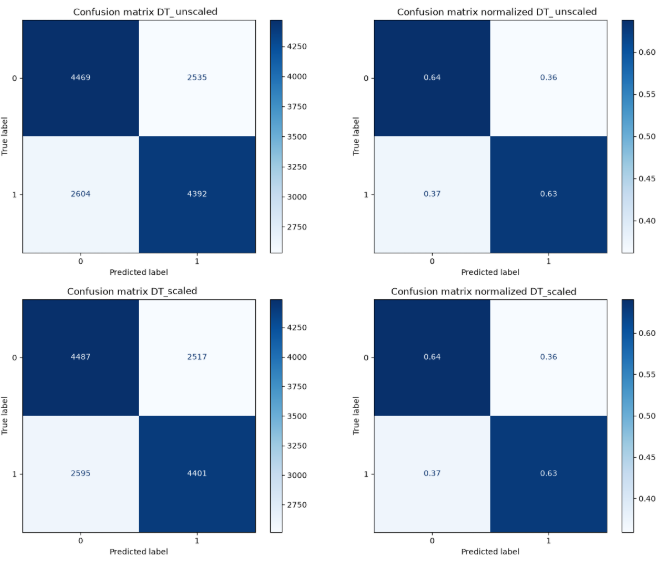
\includegraphics[width=0.85\linewidth,height=\textheight,keepaspectratio]{../res/ML_compar/Train/ML_compar_p_DT_confusion_matrix_corr.png}

}

\caption{\label{fig-aligned-vs-time}Matriz de confusión de DT en ambas
modalidades del escalamiento de datos.}

\end{figure}%

Como ya nos adelantaba el reporte de clasificación, las estadísticas no
varían entre modelos elegidos ni entre clases, siendo igual de sensible
para la clase 1 como para la 0 con unas proporciones relativamente bajas
de 0.64.

\newpage

\paragraph{RF}\label{rf}

\begin{figure}[H]

\centering{

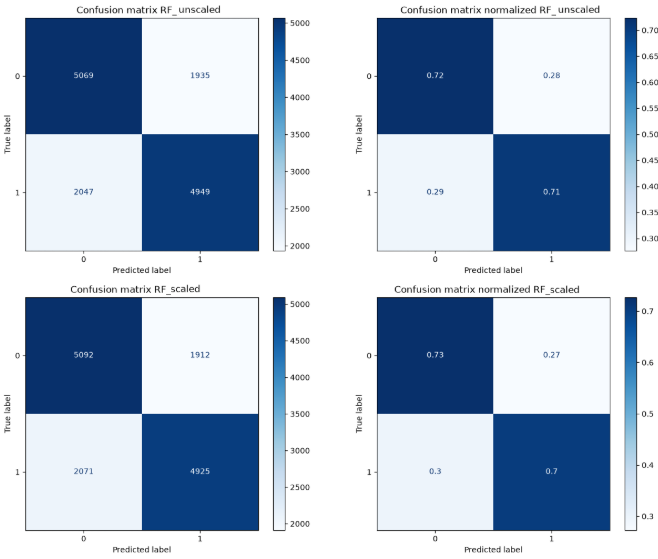
\includegraphics[width=0.85\linewidth,height=\textheight,keepaspectratio]{../res/ML_compar/Train/ML_compar_p_RF_confusion_matrix_corr.png}

}

\caption{\label{fig-aligned-vs-time}Matriz de confusión de RF en ambas
modalidades del escalamiento de datos.}

\end{figure}%

Al igual que los árboles de decisión, la diferencia entre modelos es muy
baja, así como entre clases, siendo el desempeño del modelo escalado
mejor con proporciones superiores al DT.

\newpage

\paragraph{SVM}\label{svm}

\begin{figure}[H]

\centering{

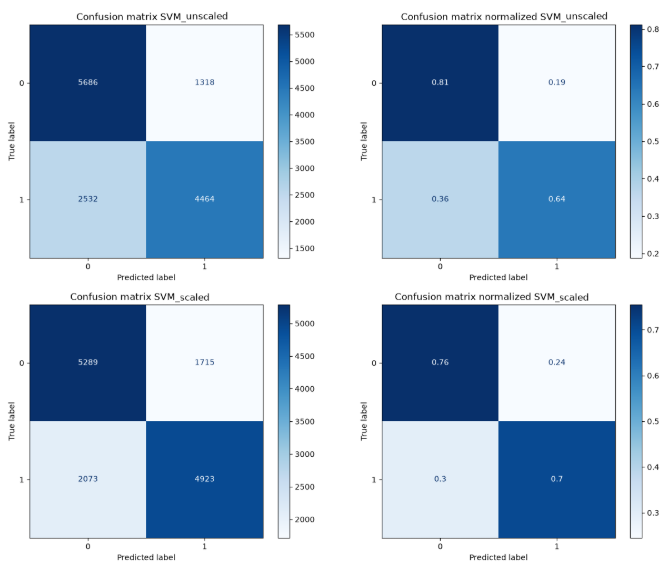
\includegraphics[width=0.85\linewidth,height=\textheight,keepaspectratio]{../res/ML_compar/Train/ML_compar_p_SVM_confusion_matrix_corr.png}

}

\caption{\label{fig-aligned-vs-time}Matriz de confusión de SVM en ambas
modalidades del escalamiento de datos.}

\end{figure}%

En el caso de los dos SVM, se puede observar cómo el rendimiento entre
ambos modelos sí es distinto, particularmente en la predicción de la
clase 1 (con cardiopatía), siendo el modelo escalado aquel con mejor
desempeño y relativamente similar al RF.

\newpage

\section{Discusión}\label{discusiuxf3n}

En esta comparación entre los 3 algoritmos de ML, se pudo comprobar cómo
los algoritmos de RF y SVM son superiores al DT para estos datos en
todas las métricas de clasificación evaluadas, siendo que las
diferencias entre ambas son bastante bajas, así como entre modelos
entrenados con datos escalados y sin escalar. Es relevante mencionar que
el modelo sin escalar RF fue superior en su capacidad predictiva para la
clase 1 de nuestra variable de interés, demostrando una sensibilidad de
la SVM a los datos sin escalar. Esto podría deberse a la representación
de los vectores y a la dificultad de encontrar un hiperplano en ese
modelo en específico, puesto que fue aquel con el hiperparámetro C más
alto (máximo posible en esta comparación de 10), así como el tiempo de
entrenamiento significativamente más grande de 63 hrs.

Este último punto es importante de destacar, puesto que el segundo
método con más tiempo de cómputo utilizado fue el SVM escalado, teniendo
un tiempo 7 veces mayor en comparación con ambos RF. Esto denota un
claro \emph{trade-off} entre recursos y un desempeño no tan superior
como se esperaría.

\section{Conclusión}\label{conclusiuxf3n}

En conclusión, el RF escalado surge como el mejor modelo evaluado en
términos de precisión por tiempo de cómputo, ya que, a pesar de que la
SVM escalada tuvo un mejor desempeño, parece ser más sensible a los
datos sin escalar, además de aumentar considerablemente su tiempo de
cómputo en el entrenamiento con este set de datos.

\begin{center}\rule{0.5\linewidth}{0.5pt}\end{center}

\section{Referencias:}\label{referencias}

\begin{enumerate}
\def\labelenumi{\arabic{enumi}.}
\item
  Pedregosa, F., Varoquaux, G., Gramfort, A., Michel, V., Thirion, B.,
  Grisel, O., Blondel, M., Prettenhofer, P., Weiss, R., Dubourg, V.,
  Vanderplas, J., Passos, A., Cournapeau, D., Brucher, M., Perrot, M.,
  \& Duchesnay, E. (2011). \emph{Scikit-learn: Machine Learning in
  Python}. Journal of Machine Learning Research, 12, 2825--2830.
\item
  Greener, J. G., Kandathil, S. M., Moffat, L., \& Jones, D. T. (2021).
  \emph{A guide to machine learning for biologists}. Nature Reviews
  Molecular Cell Biology, 23(1), 40-55.
  https://doi.org/10.1038/s41580-021-00407-0
\end{enumerate}




\end{document}
